% **************************************************************************************************
% ** SPSC Report and Thesis Template
% **************************************************************************************************
%
% ***** Authors *****
% Daniel Arnitz, Paul Meissner, Stefan Petrik
% Signal Processing and Speech Communication Laboratory (SPSC)
% Graz University of Technology (TU Graz), Austria
%
% ***** Changelog *****
% 0.1   2010-01-25   extracted from report template by Daniel Arnitz (not ready yet)
% 0.2   2010-02-08   added thesis titlepage and modified layout (not ready yet)
% 0.3   2010-02-18   added TUG logo and statutory declaration
% 0.4   2010-02-18   moved the information fields below % **************************************************************************************************
% ** SPSC Report and Thesis Template
% **************************************************************************************************
%
% ***** Authors *****
% Daniel Arnitz, Paul Meissner, Stefan Petrik
% Signal Processing and Speech Communication Laboratory (SPSC)
% Graz University of Technology (TU Graz), Austria
%
% ***** Changelog *****
%
% ***** Todo *****
%
% **************************************************************************************************



\documentclass[%
a4paper,% !!! ATTENTION: geometry package below !!!
\Twosided,% !!! ATTENTION: geometry package below !!!
openany,% begin chapters with new right page (openright) or don't care (openany)
11pt,%
fleqn,% equations not centered, but on the left side
tablecaptionbelow,% captions below tables
% titlepage,% use title
pointlessnumbers,% do not generate point at the end of section numbers (e.g. 1.4.5 instead of 1.4.5.)
final,%
]{scrreprt}% (KOMA)

\usepackage[paper=a4paper,\Twosided,%
textheight=246mm,%
textwidth=160mm,%
heightrounded=true,% round textheight to multiple of lines (avoids overfull vboxes)
ignoreall=true,% do not include header, footer, and margins in calculations
marginparsep=5pt,% marginpar only used for signs (centered), thus only small sep. needed
marginparwidth=10mm,% prevent margin notes to be out of page
hmarginratio=2:1,% set margin ration (inner:outer for twoside) - (2:3 is default)
]{geometry}%


% master
\usepackage{ifthen}% for optional parts
\usepackage[utf8]{inputenc}% German special characters
\ifthenelse{\equal{\DocumentLanguage}{en}}{\usepackage[USenglish]{babel}}{}%
\ifthenelse{\equal{\DocumentLanguage}{de}}{\usepackage[ngerman]{babel}}{}%
\usepackage[%
headtopline,plainheadtopline,% activate all lines (header and footer)
headsepline,plainheadsepline,%
footsepline,plainfootsepline,%
footbotline,plainfootbotline,%
automark% auto update \..mark
]{scrpage2}% (KOMA)
\usepackage{makeidx}% used to make an index directory
\usepackage[]{caption}% customize captions
\usepackage{multicol}%
\usepackage[stable,bottom,hang,splitrule,multiple,symbol*]{footmisc}% customize footnotes


% text
\usepackage{varioref}% improved references
\usepackage{color}% e.g., for color boxes
\usepackage{rotating}% to rotate objects
\usepackage{gensymb}% symbols (perthousand, Celsius, ...)
\usepackage[right]{eurosym}% euro symbol on the right side (51 EUR)
\usepackage[normalem]{ulem}% cross-out, strike-out, underlines (normalem: keep \emph italic)
%\usepackage[safe]{textcomp}% loading in safe mode to avoid problems (see LaTeX companion)
%\usepackage[geometry,misc]{ifsym}% technical symbols
\usepackage{remreset}%\@removefromreset commands (e.g., for continuous footnote numbering)
\usepackage[%
breaklinks=true,% allow line break in links
colorlinks=true,% if false: framed link
linkcolor=black,anchorcolor=black,citecolor=black,filecolor=black,%
menucolor=black,urlcolor=black]{hyperref}% hyperlinks for references


% math
\usepackage{amsmath,amssymb,amstext,bm} % use math packages
\usepackage{mathcomp}% symbols (perthousand, ...) in math mode


% graphics
\usepackage{graphicx}% use simple graphics
\usepackage{subfigure}% subfigures (a),(b),(c)... within figures
\usepackage{flafter}% place floats always after reference
\usepackage{placeins}% preventing floats from crossing a barrier
\usepackage{float}% to place floats !HERE!
\usepackage{psfrag}% replace text in eps figures


% tables
\usepackage{hhline}% hline doesn't work with colored columns, so using hhline
\usepackage{longtable}% for tables longer than one page
\usepackage{dcolumn}% for number alignment in tables
\usepackage{colortbl}% color in tables


% listings
%\usepackage{alltt}% verbatim environment with commands available
\usepackage{listings}% program code listings


% other
%\usepackage{layout}% graphical page layout (spacings)
\usepackage{xspace}% add space after macros if not followed by punctuation character
\makeindex% used for index creation

 (encoding...)
% 0.5   2010-03-02   added \ShortTitle to fix problems with long thesis titles
%                    added \ThesisType (makes the template suitable for MSc, BSc, PhD, ... Thesis)
%
% ***** Todo *****
% - Introduction/Usage
% **************************************************************************************************

% **************************************************************************************************
% basic setup
\newcommand{\DocumentType}{report} % "thesis" / "report"
\newcommand{\DocumentLanguage}{de} % "en" / "de"
\newcommand{\Twosided}{} % "twoside" / ""


% **************************************************************************************************
% template setup -- do not change these unless you know what you are doing!
% **************************************************************************************************
% ** SPSC Report and Thesis Template
% **************************************************************************************************
%
% ***** Authors *****
% Daniel Arnitz, Paul Meissner, Stefan Petrik
% Signal Processing and Speech Communication Laboratory (SPSC)
% Graz University of Technology (TU Graz), Austria
%
% ***** Changelog *****
%
% ***** Todo *****
%
% **************************************************************************************************



\documentclass[%
a4paper,% !!! ATTENTION: geometry package below !!!
\Twosided,% !!! ATTENTION: geometry package below !!!
openany,% begin chapters with new right page (openright) or don't care (openany)
11pt,%
fleqn,% equations not centered, but on the left side
tablecaptionbelow,% captions below tables
% titlepage,% use title
pointlessnumbers,% do not generate point at the end of section numbers (e.g. 1.4.5 instead of 1.4.5.)
final,%
]{scrreprt}% (KOMA)

\usepackage[paper=a4paper,\Twosided,%
textheight=246mm,%
textwidth=160mm,%
heightrounded=true,% round textheight to multiple of lines (avoids overfull vboxes)
ignoreall=true,% do not include header, footer, and margins in calculations
marginparsep=5pt,% marginpar only used for signs (centered), thus only small sep. needed
marginparwidth=10mm,% prevent margin notes to be out of page
hmarginratio=2:1,% set margin ration (inner:outer for twoside) - (2:3 is default)
]{geometry}%


% master
\usepackage{ifthen}% for optional parts
\usepackage[utf8]{inputenc}% German special characters
\ifthenelse{\equal{\DocumentLanguage}{en}}{\usepackage[USenglish]{babel}}{}%
\ifthenelse{\equal{\DocumentLanguage}{de}}{\usepackage[ngerman]{babel}}{}%
\usepackage[%
headtopline,plainheadtopline,% activate all lines (header and footer)
headsepline,plainheadsepline,%
footsepline,plainfootsepline,%
footbotline,plainfootbotline,%
automark% auto update \..mark
]{scrpage2}% (KOMA)
\usepackage{makeidx}% used to make an index directory
\usepackage[]{caption}% customize captions
\usepackage{multicol}%
\usepackage[stable,bottom,hang,splitrule,multiple,symbol*]{footmisc}% customize footnotes


% text
\usepackage{varioref}% improved references
\usepackage{color}% e.g., for color boxes
\usepackage{rotating}% to rotate objects
\usepackage{gensymb}% symbols (perthousand, Celsius, ...)
\usepackage[right]{eurosym}% euro symbol on the right side (51 EUR)
\usepackage[normalem]{ulem}% cross-out, strike-out, underlines (normalem: keep \emph italic)
%\usepackage[safe]{textcomp}% loading in safe mode to avoid problems (see LaTeX companion)
%\usepackage[geometry,misc]{ifsym}% technical symbols
\usepackage{remreset}%\@removefromreset commands (e.g., for continuous footnote numbering)
\usepackage[%
breaklinks=true,% allow line break in links
colorlinks=true,% if false: framed link
linkcolor=black,anchorcolor=black,citecolor=black,filecolor=black,%
menucolor=black,urlcolor=black]{hyperref}% hyperlinks for references


% math
\usepackage{amsmath,amssymb,amstext,bm} % use math packages
\usepackage{mathcomp}% symbols (perthousand, ...) in math mode


% graphics
\usepackage{graphicx}% use simple graphics
\usepackage{subfigure}% subfigures (a),(b),(c)... within figures
\usepackage{flafter}% place floats always after reference
\usepackage{placeins}% preventing floats from crossing a barrier
\usepackage{float}% to place floats !HERE!
\usepackage{psfrag}% replace text in eps figures


% tables
\usepackage{hhline}% hline doesn't work with colored columns, so using hhline
\usepackage{longtable}% for tables longer than one page
\usepackage{dcolumn}% for number alignment in tables
\usepackage{colortbl}% color in tables


% listings
%\usepackage{alltt}% verbatim environment with commands available
\usepackage{listings}% program code listings


% other
%\usepackage{layout}% graphical page layout (spacings)
\usepackage{xspace}% add space after macros if not followed by punctuation character
\makeindex% used for index creation


\input{./base/layout_\DocumentType}
% **************************************************************************************************
% ** SPSC Report and Thesis Template
% **************************************************************************************************
%
% ***** Authors *****
% Daniel Arnitz, Paul Meissner, Stefan Petrik
% Signal Processing and Speech Communication Laboratory (SPSC)
% Graz University of Technology (TU Graz), Austria
%
% ***** Changelog *****
%
% ***** Todo *****
%
% **************************************************************************************************



% **************************************************************************************************
% * SECTIONING AND TEXT
% **************************************************************************************************

% new chapter, section, ... plus a few addons
%   part
\newcommand{\newpart}[2]{\FloatBarrier\cleardoublepage\part{#1}\label{part:#2}}%
%   chapter
\newcommand{\newchapter}[2]{\FloatBarrier\chapter{#1}\label{chp:#2}}
\newcommand{\newchapterNoTOC}[2]{\FloatBarrier\stepcounter{chapter}\chapter*{#1}\label{chp:#2}}%
%   section
\newcommand{\newsection}[2]{\FloatBarrier\vspace{5mm}\section{#1}\label{sec:#2}}%
\newcommand{\newsectionNoTOC}[2]{\FloatBarrier\vspace{5mm}\stepcounter{section}\section*{#1}\label{sec:#2}}%
%   subsection
\newcommand{\newsubsection}[2]{\FloatBarrier\vspace{3mm}\subsection{#1}\label{sec:#2}}%
\newcommand{\newsubsectionNoTOC}[2]{\FloatBarrier\vspace{3mm}\stepcounter{subsection}\subsection*{#1}\label{sec:#2}}%
%   subsubsection
\newcommand{\newsubsubsection}[2]{\vspace{2mm}\subsubsection{#1}\label{sec:#2}}%
\newcommand{\newsubsubsectionNoTOC}[2]{\vspace{2mm}\stepcounter{subsubsection}\subsubsection*{#1}\label{sec:#2}}%

% next paragraph
\newcommand{\nxtpar}{\par\bigskip}

% "stylish" quotes on the right side
\newcommand{\openingquote}[2]{\hfill\parbox[t]{10cm}{\itshape\raggedleft{"#1"}\\\footnotesize -- #2}\nxtpar}%

% direct quotes
% \newenvironment{directquote}{\nxtpar\hrule}{\hrule}\hfill\litref{#1}{#2}}

% warnings and attention signs in marginpar
\newcommand{\MDanger}{\marginpar{\Huge\centering\fbox{\textbf{!}}}}%
\newcommand{\MAttention}{\marginpar{\Huge\centering\textbf{!}}}%
\newcommand{\MHint}{\marginpar{\Huge\centering\textbf{\checkmark}}}%
\newcommand{\MQuestion}{\marginpar{\Huge\centering\textbf{?}}}%

% same footnote number as last one
\newcommand{\lastfootnotemark}{\addtocounter{footnote}{-1}\footnotemark}%

% value-unit commands (for 457 kHz, etc)
\newcommand{\vu}[2]{\mbox{$#1\,\text{#2}$}} % "value~unit" ... prevents e.g. 456 \linebreak mV
\newcommand{\vuc}[3]{\mbox{$#1\,\text{#2}\;#3\,\%$}} % "value~unit~tolerance-per-cent"
\newcommand{\vum}[3]{\mbox{$#1\,\text{#2}\;#3\,\perthousand$}} % "value~unit~tolerance-per-mil"

% reminders
\newcommand{\reminder}[1]{\colorbox{red}{#1}\xspace}%
\newcommand{\rem}{\reminder{(...)}}%
\newcommand{\remq}{\reminder{???}}%
\newcommand{\uc}{\nxtpar\colorbox{yellow}{... under construction ...}\nxtpar}%

% misc
\newcommand{\pwd}{.} % present working directory (can be used to create relativ paths per part, etc.)


% **************************************************************************************************
% * MATH
% **************************************************************************************************

% highlighting
\newcommand{\vm}[1]{\bm{#1}}% vector or matrix

% operators
\newcommand{\E}[1]{\text{E}\!\left\{#1\right\}}% expectation operator
\newcommand{\var}[1]{\text{var}\!\left\{#1\right\}}% variance operator
\renewcommand{\ln}[1]{\text{ln}\!\left(#1\right)}% natural logarithm
\newcommand{\ld}[1]{\text{ld}\!\left(#1\right)}% logarithm base 2
\renewcommand{\log}[1]{\text{log}\!\left(#1\right)}% logarithm (base 10)
\newcommand{\logb}[2]{\text{log}_{#1}\!\left(#2\right)}% logarithm base ...
\newcommand{\avgvar}[1]{\overline{\text{var}}\!\left\{#1\right\}}% average variance operator
\renewcommand{\Re}[1]{\text{Re}\!\left\{#1\right\}}% real part
\renewcommand{\Im}[1]{\text{Im}\!\left\{#1\right\}}% imaginary part

% other
\newcommand{\conj}{^\ast}% conjugate complex
\newcommand{\mtx}[2]{\left[\begin{array}{#1}#2\end{array}\right]}%vector/matrix


% **************************************************************************************************
% * FLOATS (FIGURES, TABLES, LISTINGS, ...)
% **************************************************************************************************

% figures without frames
%   standard
\newcommand{\fig}[3]{\begin{figure}\centering\includegraphics[width=\textwidth]{#1}\caption{#2}\label{fig:#3}\end{figure}}%
%   with controllable parameters
\newcommand{\figc}[4]{\begin{figure}\centering\includegraphics[#1]{#2}\caption{#3}\label{fig:#4}\end{figure}}%
%   two subfigures
\newcommand{\twofig}[6]{\begin{figure}\centering%
\subfigure[#2]{\includegraphics[width=0.495\textwidth]{#1}}%
\subfigure[#4]{\includegraphics[width=0.495\textwidth]{#3}}%
\caption{#5}\label{fig:#6}\end{figure}}%
%   two subfigures and controllable parameters
\newcommand{\twofigc}[8]{\begin{figure}\centering%
\subfigure[#3]{\includegraphics[#1]{#2}}%
\subfigure[#6]{\includegraphics[#4]{#5}}%
\caption{#7}\label{fig:#8}\end{figure}}%

% framed figures
%   standard
\newcommand{\figf}[3]{\begin{figure}\centering\fbox{\includegraphics[width=\textwidth]{#1}}\caption{#2}\label{fig:#3}\end{figure}}%
%   with controllable parameters
\newcommand{\figcf}[4]{\begin{figure}\centering\fbox{\includegraphics[#1]{#2}}\caption{#3}\label{fig:#4}\end{figure}}%
%   two subfigures
\newcommand{\twofigf}[6]{\begin{figure}\centering%
\fbox{\subfigure[#2]{\includegraphics[width=0.495\textwidth]{#1}}}%
\fbox{\subfigure[#4]{\includegraphics[width=0.495\textwidth]{#3}}}%
\caption{#5}\label{fig:#6}\end{figure}}%
%   two subfigures and controllable parameters
\newcommand{\twofigcf}[8]{\begin{figure}\centering%
\fbox{\subfigure[#3]{\includegraphics[#1]{#2}}}%
\fbox{\subfigure[#6]{\includegraphics[#4]{#5}}}%
\caption{#7}\label{fig:#8}\end{figure}}%

% listings
\newcommand{\filelisting}[4]{\lstinputlisting[print=true,language=#1,caption={#3},label={lst:#4}]{#2}}

% preserve backslash for linebreaks in tables (ragged... redefines \\, thus it has to be preserved)
\newcommand{\pbs}[1]{\let\temp=\\#1\let\\=\temp}%

\graphicspath{{./drawings/}{./plots/}{./images/}}
% **************************************************************************************************
% ATTENTION: Make sure that makeindex is set to -s "./base/index.sty"
% **************************************************************************************************

% uncomment to get watermarks:
% \usepackage[first,bottom,light,draft]{draftcopy}
% \draftcopyName{ENTWURF}{160}


% **************************************************************************************************
% information fields

% general
\newcommand{\DocumentTitle}{Computational Intelligence UE}
\newcommand{\DocumentSubtitle}{Homework 2: Gradient Descent}
\newcommand{\ShortTitle}{CI Homework 2} % used in headers (keep short!)
\newcommand{\DocumentAuthor}{Thomas Ebner, Raphael Hoheneder, Stefan N\"ohmer}
\newcommand{\DocumentDate}{Graz, \today}
%    for thesis only (will be ignored for reports)
\newcommand{\ThesisType}{Master's Thesis}
\newcommand{\Organizations}{Signal Processing and Speech Communications Laboratory \\ Graz University of Technology \\[1cm] on behalf of \\ Some Company} % SPSC \\ TUG \\[1cm] on behalf of \\ A Nice Company
\newcommand{\Advisors}{Dipl.-Ing. Dr. Assoc.Prof. Klaus Witrisal \\ Dipl.-Ing. Paul Meissner} % Advisor 1 \\ Advisor 2 \\ ...
\newcommand{\Supervisors}{Univ.-Prof. Dipl.-Ing. Dr.techn. Gernot Kubin}

% revision number
\newcommand{\RevPrefix}{alpha~}
\newcommand{\RevLarge}{1}
\newcommand{\RevSmall}{1}

% confidential?
\newcommand{\ConfidNote}{confidential}% {"confidential", "eyes only", ...}

% short command for vectors
\newcommand{\vect}[1]{\mathbf{#1}}


\begin{document}

%listingstyle:
\definecolor{orange}{rgb}{0.75,0.65,0}
\definecolor{gruen}{rgb}{0,0.5,0}
\definecolor{listinggray}{gray}{0.97}
\definecolor{listingshadow}{gray}{0.2}
\lstloadlanguages{Matlab}
\lstset{frame=shadowbox,
		rulesepcolor=\color{listingshadow},
		numbers=left,
		basicstyle=\scriptsize\ttfamily,
		numberstyle=\tiny,
		keywordstyle=\color{blue}\bfseries, % bold black keywords
		identifierstyle=, % nothing happens
		commentstyle=\color{gruen}, % comments
		stringstyle=\color{orange}, % typewriter type for strings
		showstringspaces=false,
		tabsize=4,
		backgroundcolor=\color{listinggray}
        }

% **************************************************************************************************
% titlepage
\input{./base/titlepage_\DocumentType}

% statutory declaration for theses
\ifthenelse{\equal{\DocumentType}{thesis}}{% **************************************************************************************************
% ** SPSC Report and Thesis Template
% **************************************************************************************************
%
% ***** Authors *****
% Daniel Arnitz, Paul Meissner, Andreas Laesser, Stefan Petrik
% Signal Processing and Speech Communication Laboratory (SPSC)
% Graz University of Technology (TU Graz), Austria
%
% ***** Changelog *****
% 0.1   2010-02-18   created
% 0.2   2010-03-02   added German declaration
%
% ***** Todo *****
% **************************************************************************************************

\cleardoublepage
\pagestyle{empty}\pagenumbering{roman}

\vspace*{1cm}

% English
\ifthenelse{\equal{\DocumentLanguage}{en}}{
\begin{center}\Large\bfseries Statutory Declaration\end{center}\vspace*{1cm}
\noindent I declare that I have authored this thesis independently, that I have not used other than the declared sources$/$resources, and that I have explicitly marked all material which has been quoted either literally or by content from the used sources.
\par\vspace*{4cm}
\centerline{
\begin{tabular}{m{1.5cm}cm{1.5cm}m{3cm}m{1.5cm}cm{1.5cm}}
\cline{1-3} \cline{5-7}
 & date & & & & (signature) &\\
\end{tabular}}
}

% German
\ifthenelse{\equal{\DocumentLanguage}{de}}{
\begin{center}\Large\bfseries Eidesstattliche Erkl�rung\end{center}\vspace*{1cm}
Ich erkl�re an Eides statt, dass ich die vorliegende Arbeit selbstst�ndig verfasst, andere als die angegebenen Quellen$/$Hilfsmittel nicht benutzt, und die den benutzten Quellen w�rtlich und inhaltlich entnommene Stellen als solche kenntlich gemacht habe.
\par\vspace*{4cm}
\centerline{
\begin{tabular}{m{1.5cm}cm{1.5cm}m{3cm}m{1.5cm}cm{1.5cm}}
\cline{1-3} \cline{5-7}
 & Graz, am & & & & (Unterschrift) &\\
\end{tabular}}
}

}{}


% **************************************************************************************************
% **************************************************************************************************
% user-defined part

\chapter{Homework: Gradient Descent}
\section{Gradient Descent, Impulse term and adaptive learning rates}
Folgende Funktion ist gegeben:

$$ f(w_1, w_2) = -2 e^{-20(0.5(w_1-1)^2+(w_2-1)^2)} - e^{-0.1(4(w_1+1)^2 + 0.5w_2^2)} $$

Für den Gradient Descent Algorithmus wird die Ableitung dieses Ausdrucks gebraucht:

$$ grad(f) = \begin{bmatrix} \frac{\partial f}{\partial w_1} \\ \frac{\partial f}{\partial w_2} \end{bmatrix} = \begin{bmatrix} 40 (w_1 - 1) e^{-20(0.5(w_1-1)^2+(w_2-1)^2)} + 0.8 (w_1 + 1) e^{-0.1(4(w_1+1)^2 + 0.5w_2^2)} \\ 80 (w_2 - 1) e^{-20(0.5(w_1-1)^2+(w_2-1)^2)} + 0.1 w_2 e^{-0.1(4(w_1+1)^2 + 0.5w_2^2)} \end{bmatrix} $$

Für den Standard Gradient Descent Algorithmus gilt folgende Regel für die Berechnung der Gewichte $w_1$ und $w_2$ (dargestellt durch den Vektor $ \vect{w} = \begin{bmatrix} w_1 \\ w_2 \end{bmatrix} $):

$$ \vect{w_{neu}} = \vect{w} - \eta grad(f) $$


\subsection{Standard Gradient Descent}

Für diese Variante gilt die Beziehung $ \vect{w_{neu}} = \vect{w} - \eta grad(f) $. Der geschriebene \textsc{Matlab}-Code befindet sich im Anhang.

Die folgenden Abbildungen stellen die Entwicklung des Gewichtsvektors $\vect{w}$ dar:

\begin{itemize}
  \item Abbildung~\ref{fig:path_w01_eta02} zeigt den Verlauf von $\vect{w}$ für $\vect{w_0} = \begin{bmatrix} 2 \\ 0.5 \end{bmatrix}$ und $\eta = 0.2$
  \item Abbildung~\ref{fig:path_w01_eta015} zeigt den Verlauf von $\vect{w}$ für $\vect{w_0} = \begin{bmatrix} 2 \\ 0.5 \end{bmatrix}$ und $\eta = 0.15$
  \item Abbildung~\ref{fig:path_w01_eta01} zeigt den Verlauf von $\vect{w}$ für $\vect{w_0} = \begin{bmatrix} 2 \\ 0.5 \end{bmatrix}$ und $\eta = 0.1$
  \item Abbildung~\ref{fig:path_w01_eta005} zeigt den Verlauf von $\vect{w}$ für $\vect{w_0} = \begin{bmatrix} 2 \\ 0.5 \end{bmatrix}$ und $\eta = 0.05$
  \item Abbildung~\ref{fig:error_w01} zeigt den Verlauf von $f(\vect{w})$ mit $\vect{w_0} = \begin{bmatrix} 2 \\ 0.5 \end{bmatrix}$ für alle $\eta = \{0.2, 0.15, 0.1, 0.05\}$
  \item Abbildung~\ref{fig:path_w02_eta02} zeigt den Verlauf von $\vect{w}$ für $\vect{w_0} = \begin{bmatrix} -0.2 \\ -0.5 \end{bmatrix}$ und $\eta = 0.2$
  \item Abbildung~\ref{fig:path_w02_eta015} zeigt den Verlauf von $\vect{w}$ für $\vect{w_0} = \begin{bmatrix} -0.2 \\ -0.5 \end{bmatrix}$ und $\eta = 0.15$
  \item Abbildung~\ref{fig:path_w02_eta01} zeigt den Verlauf von $\vect{w}$ für $\vect{w_0} = \begin{bmatrix} -0.2 \\ -0.5 \end{bmatrix}$ und $\eta = 0.1$
  \item Abbildung~\ref{fig:path_w02_eta005} zeigt den Verlauf von $\vect{w}$ für $\vect{w_0} = \begin{bmatrix} -0.2 \\ -0.5 \end{bmatrix}$ und $\eta = 0.05$
  \item Abbildung~\ref{fig:error_w02} zeigt den Verlauf von $f(\vect{w})$ mit $\vect{w_0} = \begin{bmatrix} -0.2 \\ -0.5 \end{bmatrix}$ für alle $\eta = \{0.2, 0.15, 0.1, 0.05\}$
\end{itemize}

Man erkennt, dass die Entwicklung der Gewichte stark von den Anfangswerten und der Lernrate abhängt. Die ersten 4 Abbildungen (Abb.~\ref{fig:path_w01_eta02} bis Abb.~\ref{fig:path_w01_eta005}) zeigen den Verlauf für ein Anfangsgewicht, welches dem kleineren Minimum nahe liegt. Ist jedoch die Lernrate zu hoch ($\eta = \{0.2, 0.15\}$), bewegt sich der Verlauf ``zu schnell'' durch die Funktion, überspringt das kleine globale Minimum und landet im großen lokalen Minimum. Bei einer richtigen Lernrate ($\eta = 0.1$) landet der Verlauf im globalen Minimum und bleibt auch dort. Wählt man die Lernrate zu klein ($\eta = 0.05$), so ``verhungert'' der Verlauf und erreicht keines der Minima. Dieses Verhalten ist auch im Verlauf von $f(\vect{w})$ zu erkennen (Abb.~\ref{fig:error_w01}).

Bei einer anderen Wahl der Startgewichte (Abbildungen \ref{fig:path_w02_eta02} bis \ref{fig:path_w02_eta005}) erreicht der Verlauf nie das globale Minimum, da das lokale ``näher'' liegt. Im Verlauf von $f(\vect{w})$ (Abb.~\ref{fig:error_w02}) erkennt man, dass sich der Fehler umso schneller dem Minimum annähert, je größer die Lernrate ist.

Kurz gesagt: ist die Lernrate zu hoch, erreicht man zwar schnell ein Minimum, es besteht jedoch die Gefahr, dass ein Minimum, dass sich nur in einem kleinen, begrenzten Bereich befindet, übersprungen wird. Ist die Lernrate jedoch zu gering, kann die Anzahl der Iterationsschritte zu wenig sein, um überhaupt ein Minimum zu erreichen.


\begin{figure}[h!]
  \centering
  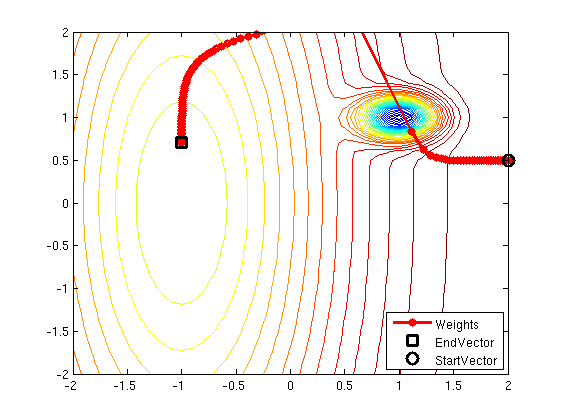
\includegraphics[width=0.8\textwidth]{./figures/211/path_w01_eta02.png}
  \caption{Verlauf von $\vect{w}$}
  \label{fig:path_w01_eta02}
\end{figure}

\begin{figure}[h!]
  \centering
  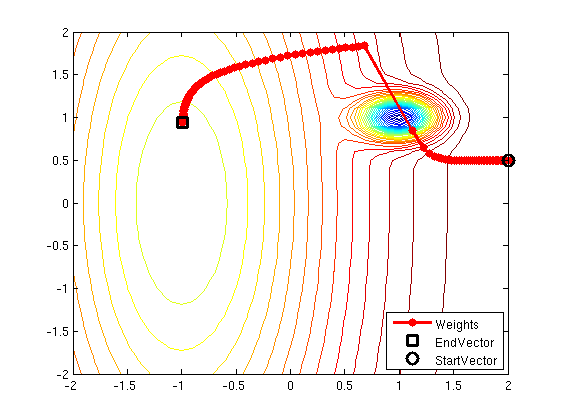
\includegraphics[width=0.8\textwidth]{./figures/211/path_w01_eta015.png}
  \caption{Verlauf von $\vect{w}$}
  \label{fig:path_w01_eta015}
\end{figure}

\begin{figure}[h!]
  \centering
  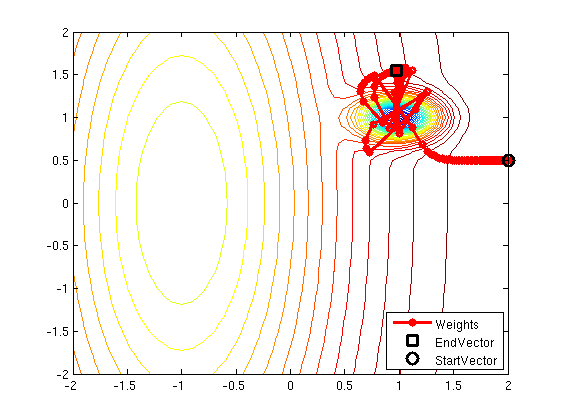
\includegraphics[width=0.8\textwidth]{./figures/211/path_w01_eta01.png}
  \caption{Verlauf von $\vect{w}$}
  \label{fig:path_w01_eta01}
\end{figure}

\begin{figure}[h!]
  \centering
  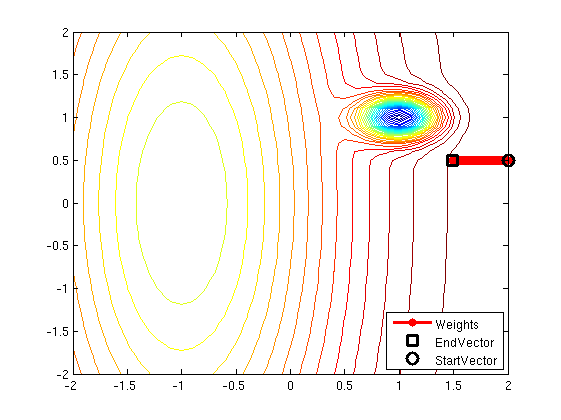
\includegraphics[width=0.8\textwidth]{./figures/211/path_w01_eta005.png}
  \caption{Verlauf von $\vect{w}$}
  \label{fig:path_w01_eta005}
\end{figure}

\begin{figure}[h!]
  \centering
  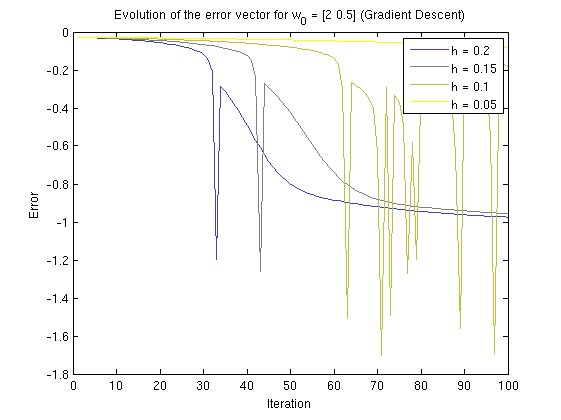
\includegraphics[width=0.8\textwidth]{./figures/211/error_w01.png}
  \caption{Verlauf von $f(\vect{w})$}
  \label{fig:error_w01}
\end{figure}

\begin{figure}[h!]
  \centering
  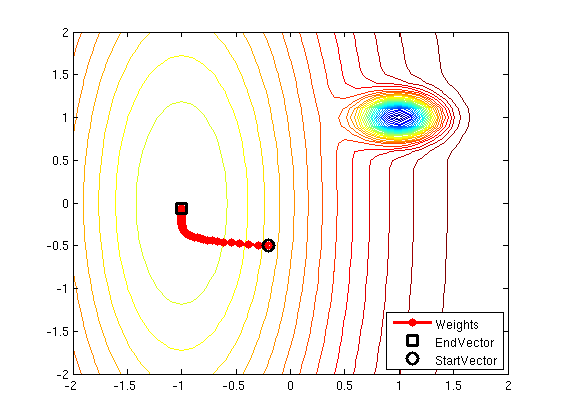
\includegraphics[width=0.8\textwidth]{./figures/211/path_w02_eta02.png}
  \caption{Verlauf von $\vect{w}$}
  \label{fig:path_w02_eta02}
\end{figure}

\begin{figure}[h!]
  \centering
  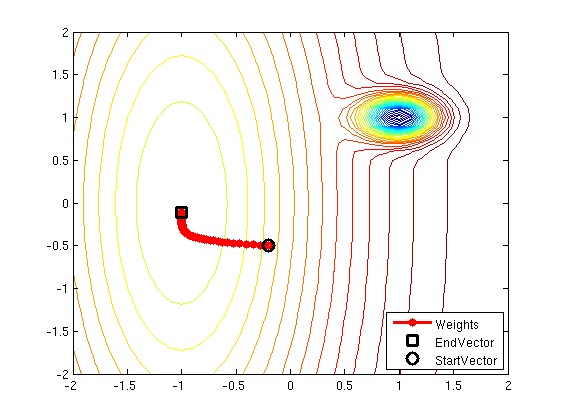
\includegraphics[width=0.8\textwidth]{./figures/211/path_w02_eta015.png}
  \caption{Verlauf von $\vect{w}$}
  \label{fig:path_w02_eta015}
\end{figure}

\begin{figure}[h!]
  \centering
  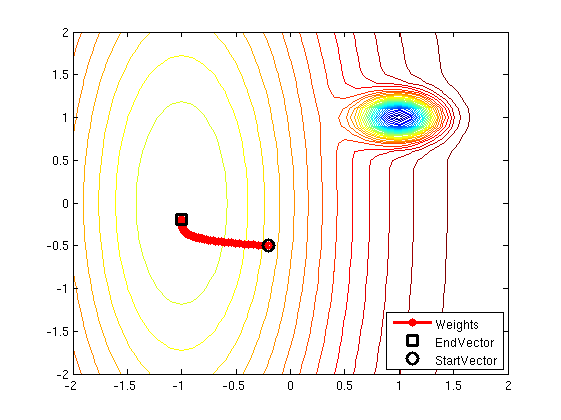
\includegraphics[width=0.8\textwidth]{./figures/211/path_w02_eta01.png}
  \caption{Verlauf von $\vect{w}$}
  \label{fig:path_w02_eta01}
\end{figure}

\begin{figure}[h!]
  \centering
  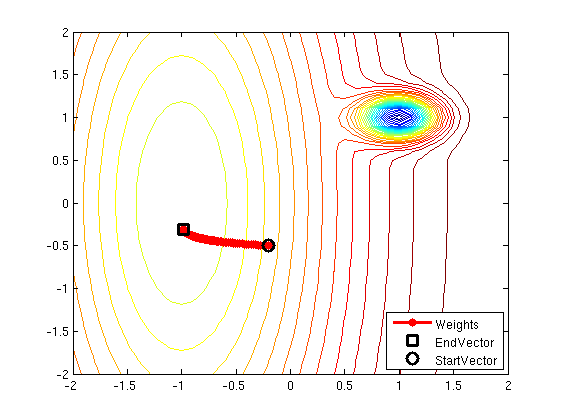
\includegraphics[width=0.8\textwidth]{./figures/211/path_w02_eta005.png}
  \caption{Verlauf von $\vect{w}$}
  \label{fig:path_w02_eta005}
\end{figure}

\begin{figure}[h!]
  \centering
  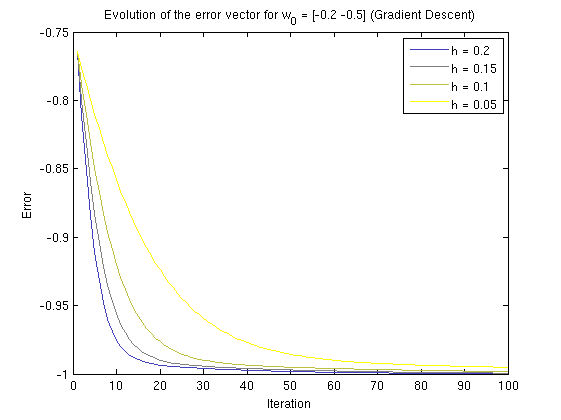
\includegraphics[width=0.8\textwidth]{./figures/211/error_w02.png}
  \caption{Verlauf von $f(\vect{w})$}
  \label{fig:error_w02}
\end{figure}

\subsection{Impulse Term}

Für diese Variante gilt die Beziehung $ \vect{w_{neu}} = \vect{w} - (1- \alpha)* \eta grad(f)  + \alpha * \Delta \vect{w_{t-1}}$. Der geschriebene \textsc{Matlab}-Code befindet sich im Anhang.

Die folgenden Abbildungen stellen die Entwicklung des Gewichtsvektors $\vect{w}$, mit einem $\alpha$ von $0.5$, dar:

\begin{itemize}
  \item Abbildung~\ref{fig:impulse_path_w01_eta02} zeigt den Verlauf von $\vect{w}$ für $\vect{w_0} = \begin{bmatrix} 2 \\ 0.5 \end{bmatrix}$ und $\eta = 0.2$
  \item Abbildung~\ref{fig:impulse_path_w01_eta015} zeigt den Verlauf von $\vect{w}$ für $\vect{w_0} = \begin{bmatrix} 2 \\ 0.5 \end{bmatrix}$ und $\eta = 0.15$
  \item Abbildung~\ref{fig:impulse_path_w01_eta01} zeigt den Verlauf von $\vect{w}$ für $\vect{w_0} = \begin{bmatrix} 2 \\ 0.5 \end{bmatrix}$ und $\eta = 0.1$
  \item Abbildung~\ref{fig:impulse_path_w01_eta005} zeigt den Verlauf von $\vect{w}$ für $\vect{w_0} = \begin{bmatrix} 2 \\ 0.5 \end{bmatrix}$ und $\eta = 0.05$
  \item Abbildung~\ref{fig:impulse_error_w01} zeigt den Verlauf von $f(\vect{w})$ mit $\vect{w_0} = \begin{bmatrix} 2 \\ 0.5 \end{bmatrix}$ für alle $\eta = \{0.2, 0.15, 0.1, 0.05\}$
  \item Abbildung~\ref{fig:impulse_path_w02_eta02} zeigt den Verlauf von $\vect{w}$ für $\vect{w_0} = \begin{bmatrix} -0.2 \\ -0.5 \end{bmatrix}$ und $\eta = 0.2$
  \item Abbildung~\ref{fig:impulse_path_w02_eta015} zeigt den Verlauf von $\vect{w}$ für $\vect{w_0} = \begin{bmatrix} -0.2 \\ -0.5 \end{bmatrix}$ und $\eta = 0.15$
  \item Abbildung~\ref{fig:impulse_path_w02_eta01} zeigt den Verlauf von $\vect{w}$ für $\vect{w_0} = \begin{bmatrix} -0.2 \\ -0.5 \end{bmatrix}$ und $\eta = 0.1$
  \item Abbildung~\ref{fig:impulse_path_w02_eta005} zeigt den Verlauf von $\vect{w}$ für $\vect{w_0} = \begin{bmatrix} -0.2 \\ -0.5 \end{bmatrix}$ und $\eta = 0.05$
  \item Abbildung~\ref{fig:impulse_error_w02} zeigt den Verlauf von $f(\vect{w})$ mit $\vect{w_0} = \begin{bmatrix} -0.2 \\ -0.5 \end{bmatrix}$ für alle $\eta = \{0.2, 0.15, 0.1, 0.05\}$
\end{itemize}

In Abb. ~\ref{fig:impulse_path_w01_eta015} sieht man, dass der Verlauf nicht mehr direkt das kleinere Minimum überspringt, sondern erst einige male um das kleine Minimum herum springt bevor der Verlauf weiter in Richtung großen Minimum weitergeht. Bei der besten Lernrate ($\eta =0.1$) wie in Abb.~\ref{fig:impulse_path_w01_eta01}, sieht man das hier nicht nur der Verlauf das globale Minimum genauer trifft sondern auch weniger darüber hinaus springt. Um das globale Minimum exakt zu treffen wären aber weitere Iterations-schritte nötig. Die Impulse Term-variante  bringt aber bei ``Verhungerung'' auch keine Verbesserung wie in Abb.~\ref{fig:impulse_path_w01_eta005} zu sehen ist. Was auch zu erwarten ist da man ja nur den Gradient mit dem vorherigen dämpft.

Wie im Vorangegangen Bsp. erreicht auch mit der Impulse Term-variante der Verlauf, mit anderen Startgewichten (Abbildungen \ref{fig:impulse_path_w02_eta02} bis \ref{fig:impulse_path_w02_eta005}), nie das globale Minimum. Mit bloßem Auge ist hier kein Unterschied erkennbar. Keine Verbesserung für ``schlechte'' gewählte Startgewichte!


Der Fehler wird bei $\eta = 0.1$ und $\vect{w_0} = \begin{bmatrix} 2 \\ 0.5 \end{bmatrix}$  klein und bleibt dann in etwa  auf dem selben Niveau, da er, wie man in Abb.~\ref{fig:impulse_path_w01_eta01} sehen kann, knapp rund um das globale Minimum herum springt.





\begin{figure}[h!]
  \centering
  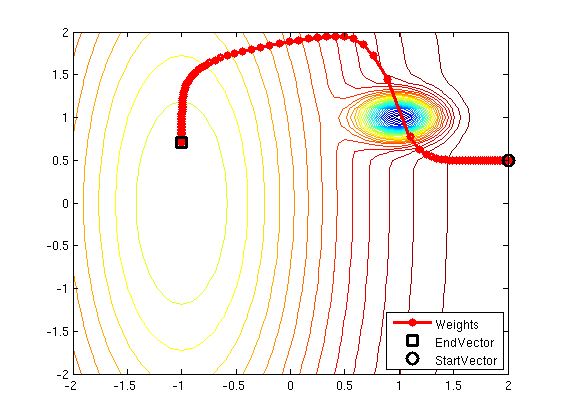
\includegraphics[width=0.8\textwidth]{./figures/212/path_w01_eta02.png}
  \caption{Verlauf von $\vect{w}$}
  \label{fig:impulse_path_w01_eta02}
\end{figure}

\begin{figure}[h!]
  \centering
  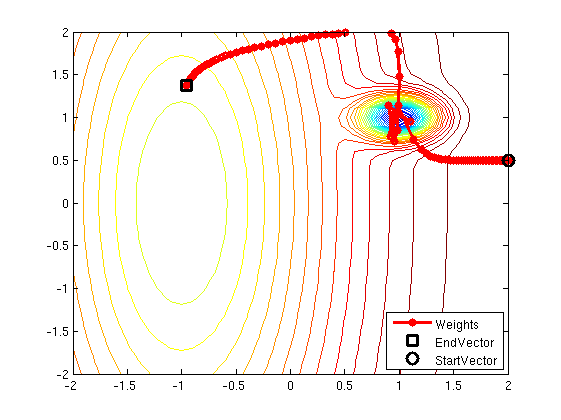
\includegraphics[width=0.8\textwidth]{./figures/212/path_w01_eta015.png}
  \caption{Verlauf von $\vect{w}$}
  \label{fig:impulse_path_w01_eta015}
\end{figure}

\begin{figure}[h!]
  \centering
  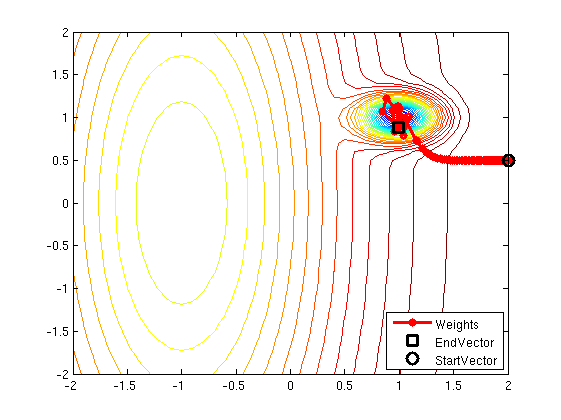
\includegraphics[width=0.8\textwidth]{./figures/212/path_w01_eta01.png}
  \caption{Verlauf von $\vect{w}$}
  \label{fig:impulse_path_w01_eta01}
\end{figure}

\begin{figure}[h!]
  \centering
  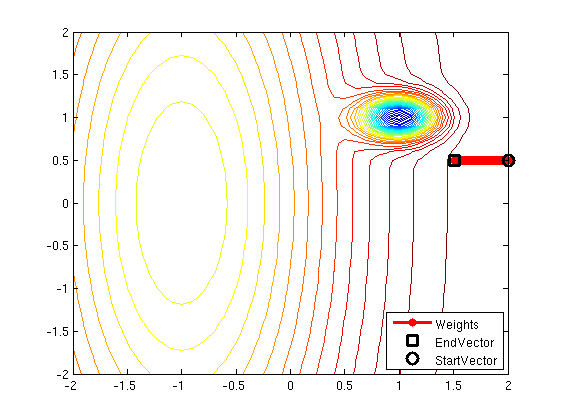
\includegraphics[width=0.8\textwidth]{./figures/212/path_w01_eta005.png}
  \caption{Verlauf von $\vect{w}$}
  \label{fig:impulse_path_w01_eta005}
\end{figure}

\begin{figure}[h!]
  \centering
  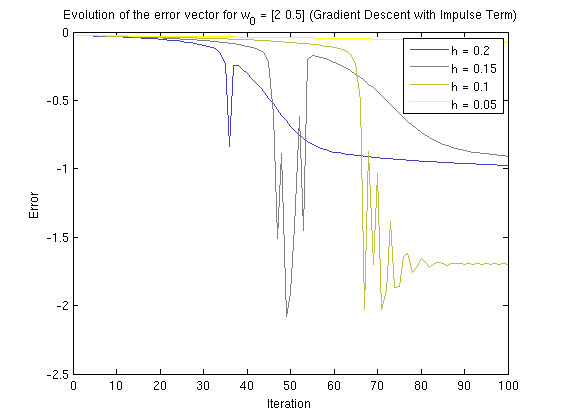
\includegraphics[width=0.8\textwidth]{./figures/212/error_w01.png}
  \caption{Verlauf von $f(\vect{w})$}
  \label{fig:impulse_error_w01}
\end{figure}

\begin{figure}[h!]
  \centering
  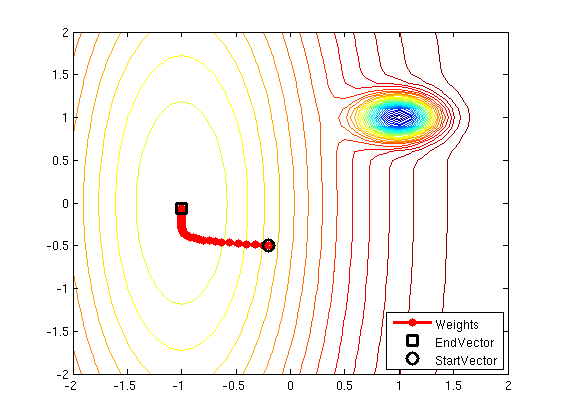
\includegraphics[width=0.8\textwidth]{./figures/212/path_w02_eta02.png}
  \caption{Verlauf von $\vect{w}$}
  \label{fig:impulse_path_w02_eta02}
\end{figure}

\begin{figure}[h!]
  \centering
  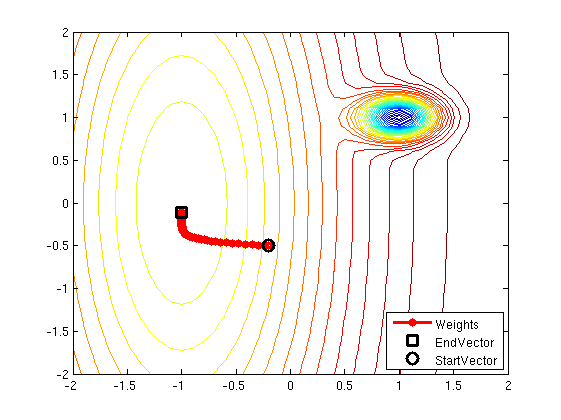
\includegraphics[width=0.8\textwidth]{./figures/212/path_w02_eta015.png}
  \caption{Verlauf von $\vect{w}$}
  \label{fig:impulse_path_w02_eta015}
\end{figure}

\begin{figure}[h!]
  \centering
  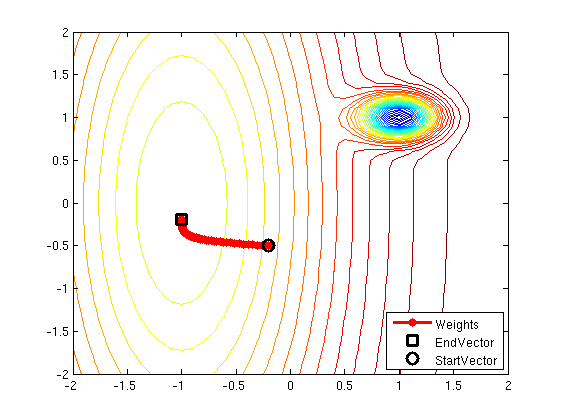
\includegraphics[width=0.8\textwidth]{./figures/212/path_w02_eta01.png}
  \caption{Verlauf von $\vect{w}$}
  \label{fig:impulse_path_w02_eta01}
\end{figure}

\begin{figure}[h!]
  \centering
  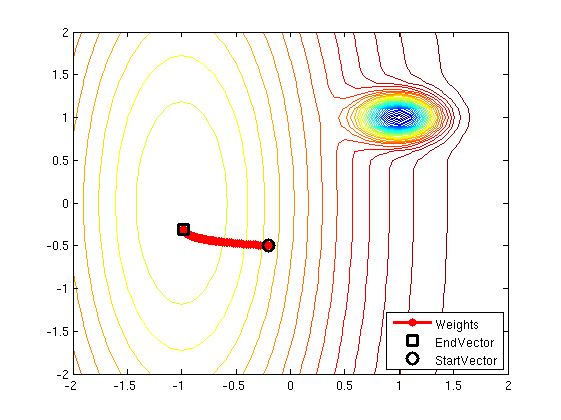
\includegraphics[width=0.8\textwidth]{./figures/212/path_w02_eta005.png}
  \caption{Verlauf von $\vect{w}$}
  \label{fig:impulse_path_w02_eta005}
\end{figure}

\begin{figure}[h!]
  \centering
  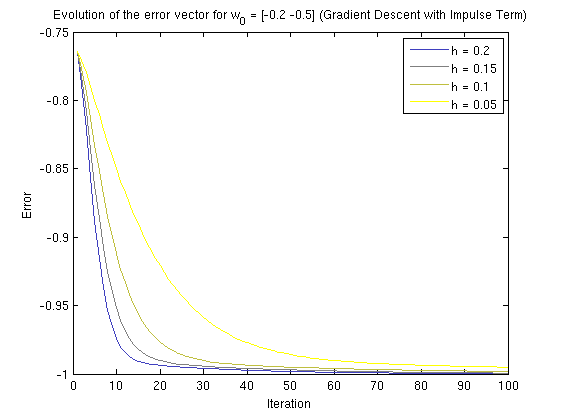
\includegraphics[width=0.8\textwidth]{./figures/212/error_w02.png}
  \caption{Verlauf von $f(\vect{w})$}
  \label{fig:impulse_error_w02}
\end{figure}

\clearpage
\newpage
\subsection{Adaptive learning rate}

Für diese Variante gilt die Beziehung $ \vect{w_{neu}} = \vect{w} - \eta \cdot grad(f)(1-\alpha) +  \alpha \cdot \vect{\Delta w_{i-1}}$. Der geschriebene \textsc{Matlab}-Code befindet sich im Anhang.

Die folgenden Abbildungen stellen die Entwicklung des Gewichtsvektors $\vect{w}$ dar:

\begin{itemize}
  \item Abbildung~\ref{fig:path_w01_eta02} zeigt den Verlauf von $\vect{w}$ für $\vect{w_0} = \begin{bmatrix} 2 \\ 0.5 \end{bmatrix}$ und $\eta = 0.2$
  \item Abbildung~\ref{fig:path_w01_eta015} zeigt den Verlauf von $\vect{w}$ für $\vect{w_0} = \begin{bmatrix} 2 \\ 0.5 \end{bmatrix}$ und $\eta = 0.15$
  \item Abbildung~\ref{fig:path_w01_eta01} zeigt den Verlauf von $\vect{w}$ für $\vect{w_0} = \begin{bmatrix} 2 \\ 0.5 \end{bmatrix}$ und $\eta = 0.1$
  \item Abbildung~\ref{fig:path_w01_eta005} zeigt den Verlauf von $\vect{w}$ für $\vect{w_0} = \begin{bmatrix} 2 \\ 0.5 \end{bmatrix}$ und $\eta = 0.05$
  \item Abbildung~\ref{fig:error_w01} zeigt den Verlauf von $f(\vect{w})$ mit $\vect{w_0} = \begin{bmatrix} 2 \\ 0.5 \end{bmatrix}$ für alle $\eta = \{0.2, 0.15, 0.1, 0.05\}$
  \item Abbildung~\ref{fig:path_w02_eta02} zeigt den Verlauf von $\vect{w}$ für $\vect{w_0} = \begin{bmatrix} -0.2 \\ -0.5 \end{bmatrix}$ und $\eta = 0.2$
  \item Abbildung~\ref{fig:path_w02_eta015} zeigt den Verlauf von $\vect{w}$ für $\vect{w_0} = \begin{bmatrix} -0.2 \\ -0.5 \end{bmatrix}$ und $\eta = 0.15$
  \item Abbildung~\ref{fig:path_w02_eta01} zeigt den Verlauf von $\vect{w}$ für $\vect{w_0} = \begin{bmatrix} -0.2 \\ -0.5 \end{bmatrix}$ und $\eta = 0.1$
  \item Abbildung~\ref{fig:path_w02_eta005} zeigt den Verlauf von $\vect{w}$ für $\vect{w_0} = \begin{bmatrix} -0.2 \\ -0.5 \end{bmatrix}$ und $\eta = 0.05$
  \item Abbildung~\ref{fig:error_w02} zeigt den Verlauf von $f(\vect{w})$ mit $\vect{w_0} = \begin{bmatrix} -0.2 \\ -0.5 \end{bmatrix}$ für alle $\eta = \{0.2, 0.15, 0.1, 0.05\}$
\end{itemize}

Vergleicht man die Abbildungen mit denen der vorhergehenden Kapitel, so fällt sofort auf, dass diese
Variante deutlich bessere Ergebnise liefert. Der Grund dafür ist, dass sobald der Fehler größer wird,
der neuberechnete Gewichtsvektor wieder verworfen wird. So ist es nicht möglich, dass sobald man sich in einem
Minima befindet, man wieder heraushüpft.

Die Wahl des Gewichtsvektors zu beginn, ist also entscheidend, in welchen Minima man landet.

\begin{figure}[h!]
  \centering
  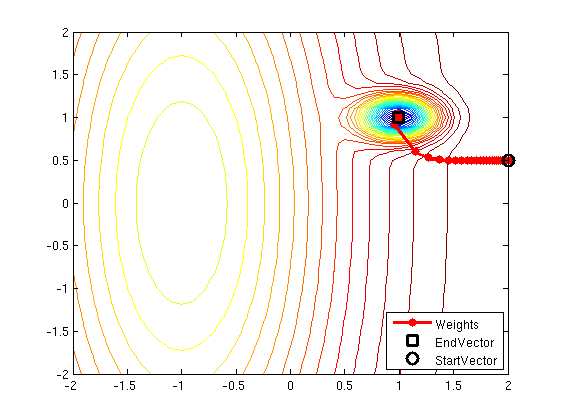
\includegraphics[width=0.8\textwidth]{./figures/213/path_w01_eta02.png}
  \caption{Verlauf von $\vect{w}$}
  \label{fig:path_w01_eta02}
\end{figure}

\begin{figure}[h!]
  \centering
  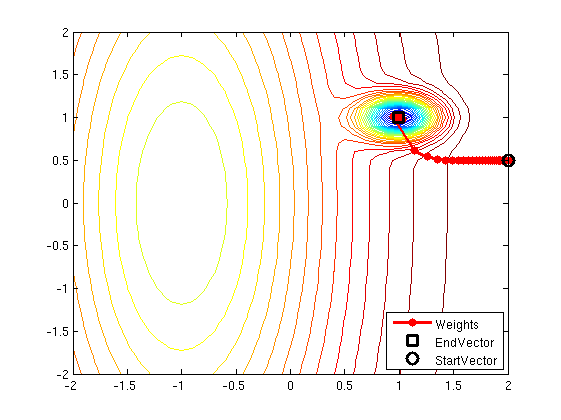
\includegraphics[width=0.8\textwidth]{./figures/213/path_w01_eta015.png}
  \caption{Verlauf von $\vect{w}$}
  \label{fig:path_w01_eta015}
\end{figure}

\begin{figure}[h!]
  \centering
  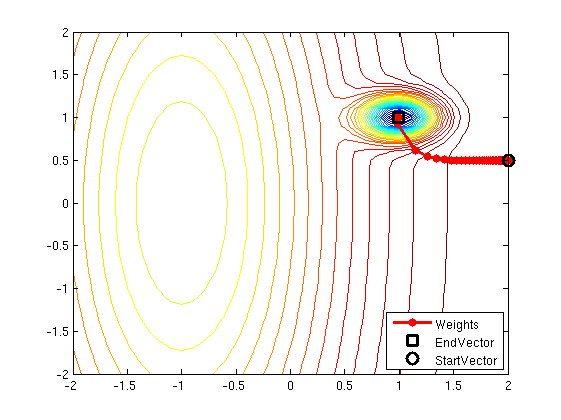
\includegraphics[width=0.8\textwidth]{./figures/213/path_w01_eta01.png}
  \caption{Verlauf von $\vect{w}$}
  \label{fig:path_w01_eta01}
\end{figure}

\begin{figure}[h!]
  \centering
  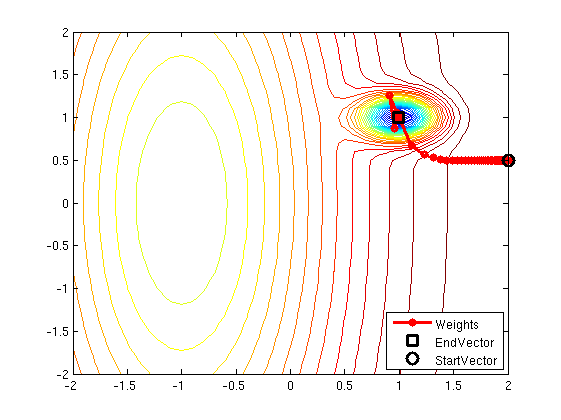
\includegraphics[width=0.8\textwidth]{./figures/213/path_w01_eta005.png}
  \caption{Verlauf von $\vect{w}$}
  \label{fig:path_w01_eta005}
\end{figure}

\begin{figure}[h!]
  \centering
  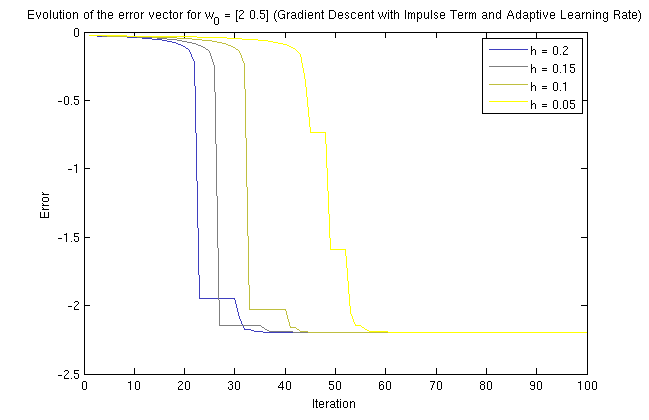
\includegraphics[width=0.8\textwidth]{./figures/213/error_w01.png}
  \caption{Verlauf von $f(\vect{w})$}
  \label{fig:error_w01}
\end{figure}

\begin{figure}[h!]
  \centering
  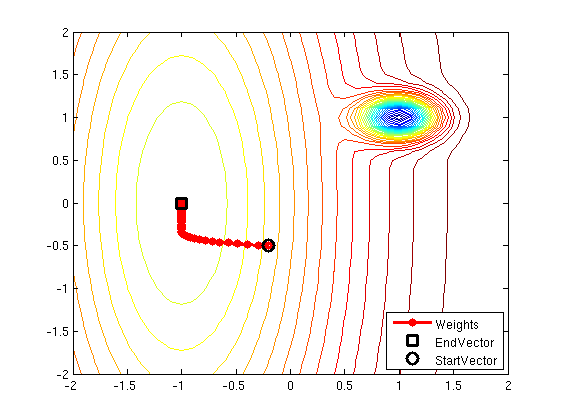
\includegraphics[width=0.8\textwidth]{./figures/213/path_w02_eta02.png}
  \caption{Verlauf von $\vect{w}$}
  \label{fig:path_w02_eta02}
\end{figure}

\begin{figure}[h!]
  \centering
  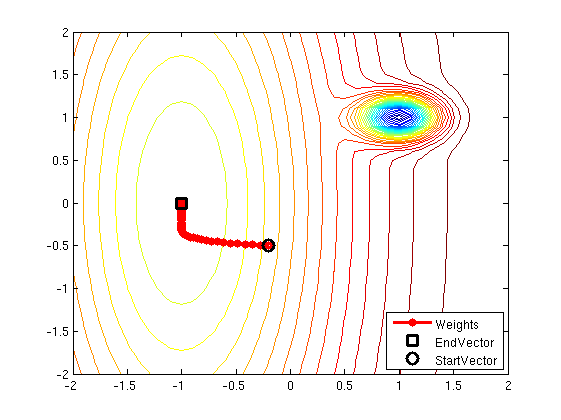
\includegraphics[width=0.8\textwidth]{./figures/213/path_w02_eta015.png}
  \caption{Verlauf von $\vect{w}$}
  \label{fig:path_w02_eta015}
\end{figure}

\begin{figure}[h!]
  \centering
  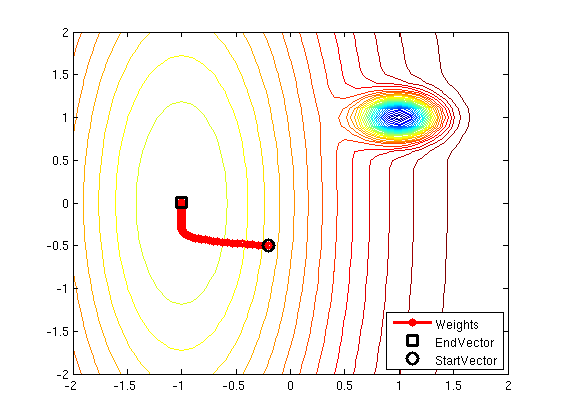
\includegraphics[width=0.8\textwidth]{./figures/213/path_w02_eta01.png}
  \caption{Verlauf von $\vect{w}$}
  \label{fig:path_w02_eta01}
\end{figure}

\begin{figure}[h!]
  \centering
  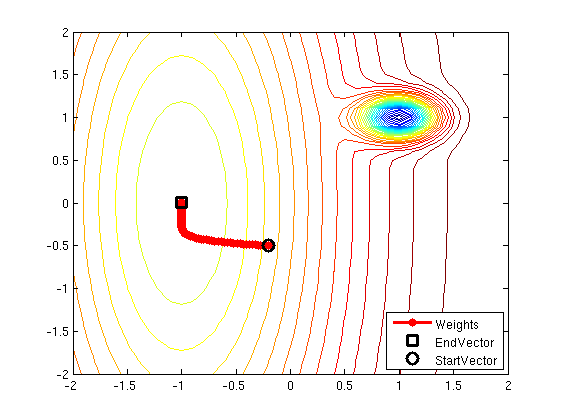
\includegraphics[width=0.8\textwidth]{./figures/213/path_w02_eta005.png}
  \caption{Verlauf von $\vect{w}$}
  \label{fig:path_w02_eta005}
\end{figure}

\begin{figure}[h!]
  \centering
  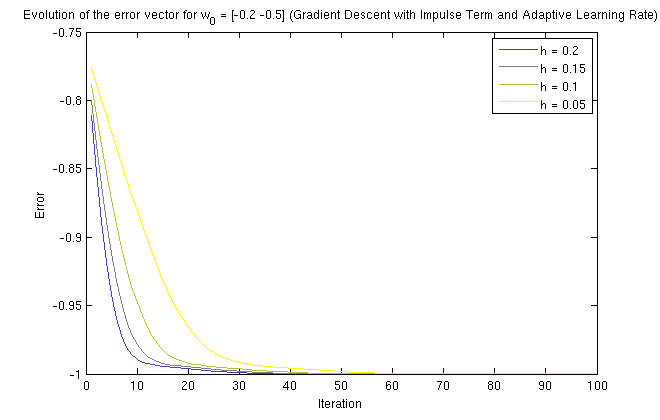
\includegraphics[width=0.8\textwidth]{./figures/213/error_w02.png}
  \caption{Verlauf von $f(\vect{w})$}
  \label{fig:error_w02}
\end{figure}

\clearpage
\newpage
\subsection{Local Minima}

Man erreicht das globale Minima nur, wenn man direkt im globalem Minima startet.
Im Endeffekt erreicht man nur in 0.059488\% der Fälle das globale Mimima. In den restlichen Fällen landet man
entweder im lokalem Minima(ebene Fläche im Plot), oder erreicht gar kein Minima(Spitzen im Plot).


\begin{figure}[h!]
  \centering
  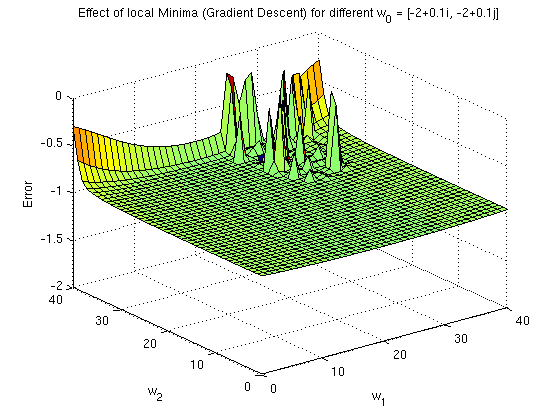
\includegraphics[width=0.8\textwidth]{./figures/214/minf.png}
  \caption{Verlauf von $\vect{w}$}
  \label{fig:minf}
\end{figure}

\clearpage
\newpage

\chapter{Listings}
\section{Standard Gradient Descent}
\lstinputlisting[language=matlab]{../implementation/hw211.m}
\section{Impulse Term}
\lstinputlisting[language=matlab]{../implementation/hw212.m}
\section{Adaptive learning rage}
\lstinputlisting[language=matlab]{../implementation/hw213.m}
\section{local minima}
\lstinputlisting[language=matlab]{../implementation/hw214.m}





% **************************************************************************************************
% **************************************************************************************************

%\appendix
%\bibliographystyle{/.base/ieeetran}
%\bibliography{_bibliography}

% place all floats and create label on last page
\FloatBarrier\label{end-of-document}
\end{document}

